%% This is free and unencumbered software released into the public domain.

%% Anyone is free to copy, modify, publish, use, compile, sell, or
%% distribute this software, either in source code form or as a compiled
%% binary, for any purpose, commercial or non-commercial, and by any
%% means.

%% In jurisdictions that recognize copyright laws, the author or authors
%% of this software dedicate any and all copyright interest in the
%% software to the public domain. We make this dedication for the benefit
%% of the public at large and to the detriment of our heirs and
%% successors. We intend this dedication to be an overt act of
%% relinquishment in perpetuity of all present and future rights to this
%% software under copyright law.

%% THE SOFTWARE IS PROVIDED "AS IS", WITHOUT WARRANTY OF ANY KIND,
%% EXPRESS OR IMPLIED, INCLUDING BUT NOT LIMITED TO THE WARRANTIES OF
%% MERCHANTABILITY, FITNESS FOR A PARTICULAR PURPOSE AND NONINFRINGEMENT.
%% IN NO EVENT SHALL THE AUTHORS BE LIABLE FOR ANY CLAIM, DAMAGES OR
%% OTHER LIABILITY, WHETHER IN AN ACTION OF CONTRACT, TORT OR OTHERWISE,
%% ARISING FROM, OUT OF OR IN CONNECTION WITH THE SOFTWARE OR THE USE OR
%% OTHER DEALINGS IN THE SOFTWARE.

%% For more information, please refer to <https://unlicense.org>
%%
\chapter{Constraint Random Verification}\label{constraintrandom}
The complexity of digital design is growing with the capacity of the silicon. A
decade ago, the industry started to move away from ``direct" testing towards
functional coverage and formal methods. In the previous chapter, the concept of
Functional Verification and Coverage Driven Verification was introduced and
explained. This chapter focuses on the generation of random stimuli for
functionally verify a device, this includes how the stimuli are produced, the
elements needed for generating exhaustible random input vectors, and how these
random inputs are optimized and tailored for the device under test. The first
part of this chapter describes Random Constraint Verification, why it is
necessary and how it is achieved in other verification languages. The second
part focuses more on the theory behind constraint solving and the mathematical
tools that allow this verification paradigm.

\section{Environment setup and requirements}
As explained in section \ref{sec:covdrivenv}, the most significant advantage of
adopting a functional coverage methodology is the possibility of exploring and
verifying the state space of a design by automatically generating input vectors
for tests. When the machine automatically generates tests, a surrounding
infrastructure responsible for probing the functional coverage and resultant
correctness must be already in place. Building the surrounding infrastructure,
including the golden-model to self-predict a random input vector's outcome, can
be time consuming \cite{spear2008systemverilog} but when the infrastructure is
in place, it allows to reach the desire verification quality in less time.
Figure \ref{fig:crv:comdirectrandom}, shows the comparison between the
approximated developing time of a reusable testbench and a traditional
testbench.

\begin{figure}[htbp]
\centering
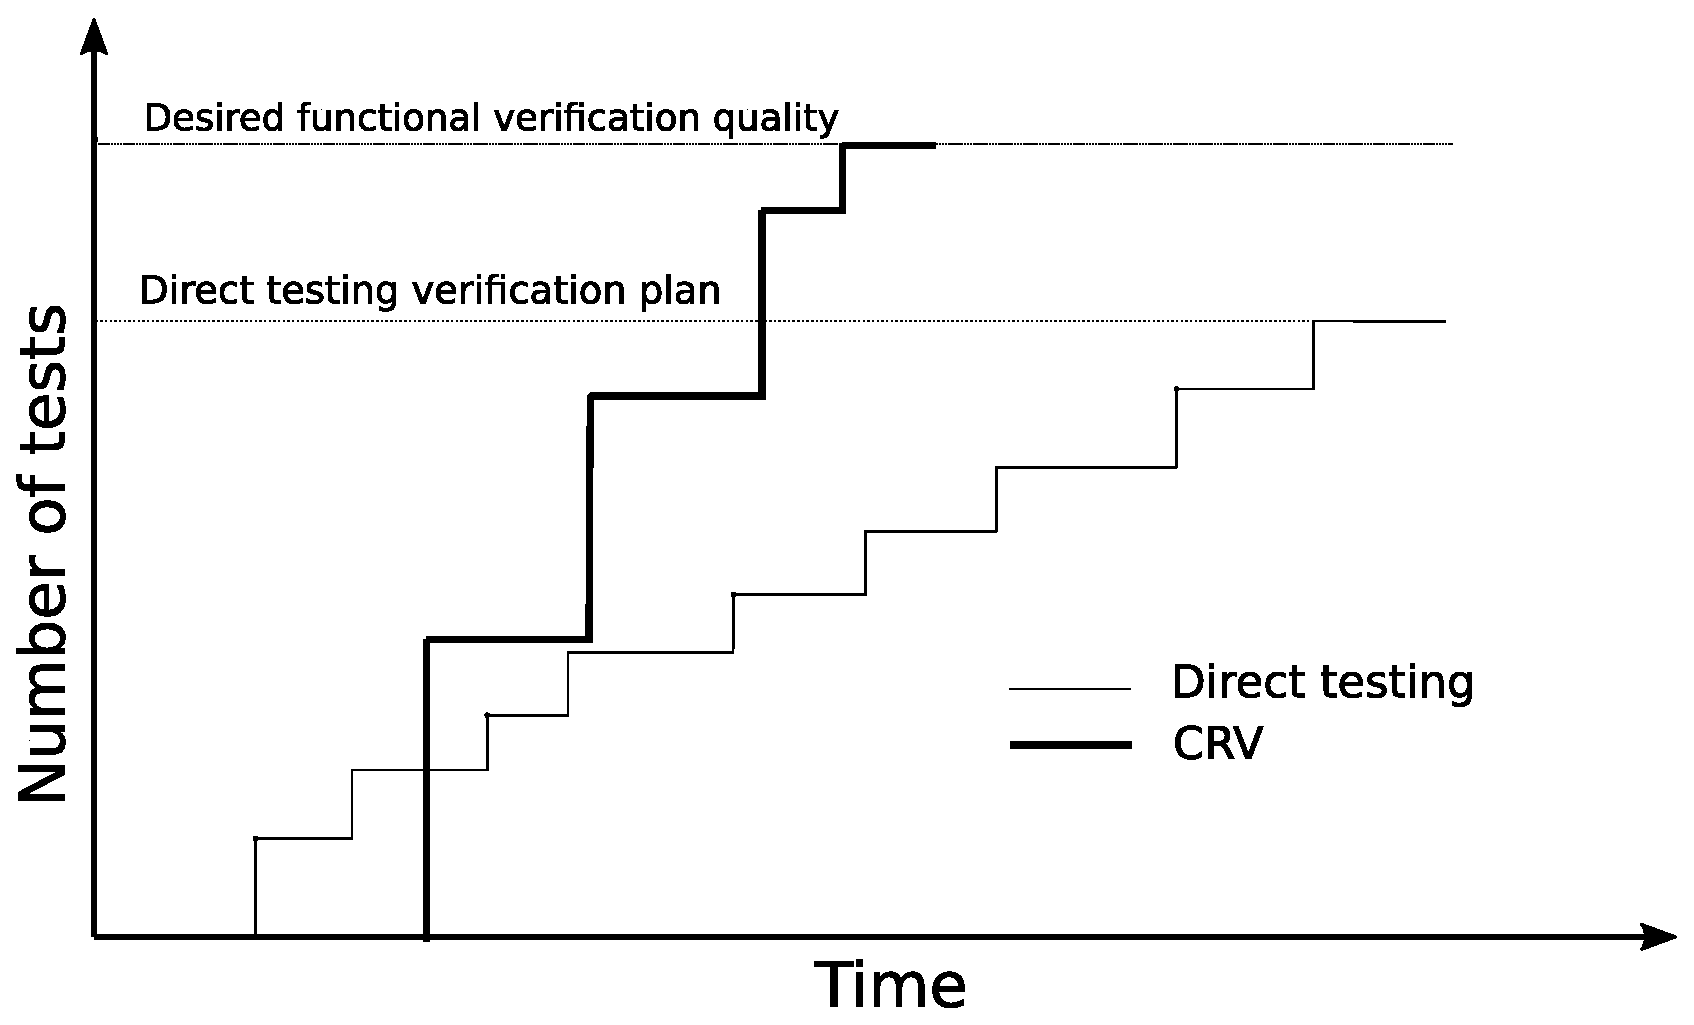
\includegraphics[width=0.6\linewidth]{pictures/Quality_testing.eps}
\caption{Constrained-random test progress over time compared to directed testing \cite{spear2008systemverilog}.}
\label{fig:crv:comdirectrandom}
\end{figure}

From \ref{fig:crv:comdirectrandom}, it is clear that the time needed to build a
flexible verification environment is higher at the beginning of the development
process but guarantees better productivity. The productivity gain is achieved by
sharing the same flexible testbench across all the machine-generated tests.
Using the machine-generated test leads to faster bug discovery than traditional
tests, especially in the initial testing phase.

When the discovery rate of bugs and the functional coverage percentage stalls
and random input vectors are no longer sufficient, the traditional approach can
be used to create tailored input vectors that reach complex parts of the model
state space.

\section{Constrained Random Stimuli}\label{sec:constrainedrandomsti}
Generally, to increase random stimuli's productivity, the input vector used to
test the devices must be a valid input vector that does not violate the design's
specification. For this reason, to avoid generating unsound stimuli that might
lead to false-negative verification results, the stimulus generator must
restrict the produced random input vector by following specific constraints
derived from the design specifications. For example, implementing a protocol
interface may only be correct for packets with a particular header, so the
stimulus generator will constrain its output to exclude all the invalid headers.

This practice of constraining the randomization output is also known as
Constraint Programming. Commonly, the random generator and the constraint are
specified on top of object-oriented data abstractions. Leveraging the
object-oriented paradigm, it allows to model the data to be randomized as
objects containing random fields and user-defined constraints. Such objects can
implicitly express the constraints inside their definition or explicitly accept
constraints passed as input parameters. Objects are the ideal data structure for
representing aggregate data types that can directly map to an input vector for
the hardware under test, for example a class encapsulates the definition of a
network packet.

The constraint random verification process can be utilized at many levels inside
the verification environment. The most primitive randomization occurs at the
hardware level, where the testbench toggles a device's pins. A second step is to
randomize the timing between the protocol requests. A higher type of
randomization can occur within each transaction and between transactions.

Figure \ref{fig:crv:alu} shows an example of an ALU component that has two 8-bit
widths unsigned operands input (\mints{a}, \mints{b}), one 2-bit width operation
input (\mints{fn}), and an 8-bit unsigned output result (\mints{c}).

\begin{figure}[htbp]
\centering
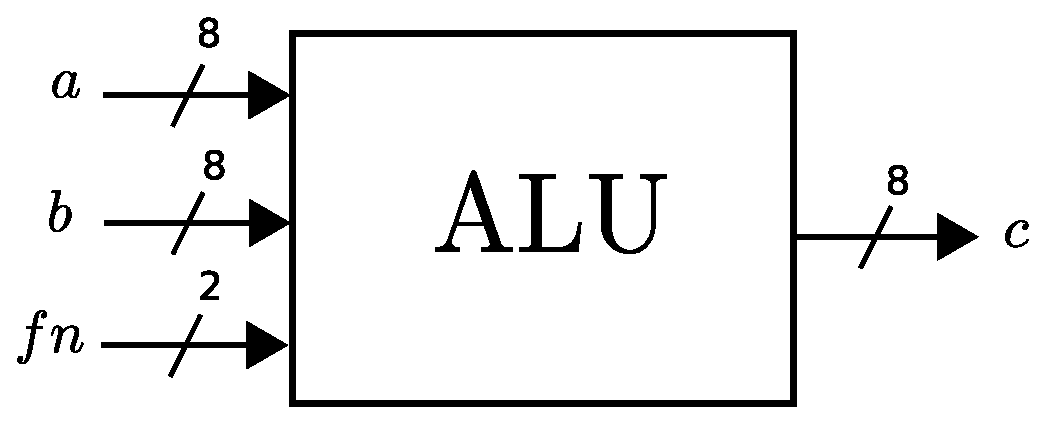
\includegraphics[width=0.4\linewidth]{pictures/ALU.eps}
\caption{8-bit ALU block diagram.}
\label{fig:crv:alu}
\end{figure}

Assuming the ALU accepts four types of operations, addition, subtractions,
bit-wise AND, and bit-wise OR, it is clear that the result will overflow or is
invalid for certain types of value, for example, when \mints{a + b > 255}. The
problem of limiting the input value of a specific transaction can be expressed
as a mathematical system of the equation that, when solved at the same time,
returns a domain of valid solution for the ALU. For the current ALU, the system
of equations that express only the valid input can be expressed as:

\begin{equation}
\mathcal{S} =
  \begin{cases}
    a + b \leq 255 \\
    a - b \geq 0\\
  \end{cases}.
\end{equation}

The system of equations $\mathcal{S}$ is composed of two equations describing a
binary constraint (two input variables) for ADD, SUB. In order to limit the
``invalid" transactions that this component receives during a test, in hardware
constraint language like SystemVerilog, it is common practice to create an
object representing a transaction containing the three ALU inputs as random
fields and constrain the randomization of the class by declaring constraints
inside it.

\begin{listing}[ht]
\begin{minted}
[
frame=lines,
framesep=2mm,
baselinestretch=1.2,
fontsize=\footnotesize,
linenos
]
{systemverilog}
class ALU_t;
    rand enum { ADD, SUB, AND, OR } fn;
    rand bit signed [7:0] a, b;
    constraint valid {
        a + b <= 255; 
        a - b >= 0;
    }
}
\end{minted}
\caption{SystemVerilog ALU transaction example.}
\label{listing:3}
\end{listing}

In line 2 and 3 of listing \ref{listing:3}, the \mints{fn} enumerator and the
(\mints{a}, \mints{b}) inputs are declared with the \mints{rand} keyword. In
line 4, a constraint name \mints{valid} is declared, and for each type of
operation, it limits the possible value. In this specific example, the
\mints{fn} input is defined as an enumerator, and thus its values are already
limited by its type. In the next section, the concept of constraint satisfaction
problems is introduced, and subsequently, in the next chapters, two different
solutions on how to solve constraint satisfaction problems in Chisel are showed.


\section{Constraint Satisfaction Problems}
One of the pillars of functional verification is constraint programming.
Constraint programming (CP) is a programming paradigm that has been developed
since the mid-1980s and emerged as a further development of logic programming.
Constraint-based programming allows constraints and their solution mechanisms to
be integrated into a programming language. Constraints are relations between
variables, and a constraint satisfaction problem describes which relations are
valid in a specific problem. With constraint programming, the user describes the
problem in a declarative way, while the solution process takes a back seat from
the user's perspective. A subset of these problems is the so-called Constraint
Satisfaction Problems (CSP), which are mathematical problems defined as a set of
objects such that their state must satisfy several constraints.

\subsubsection{Definition}\label{sec:csp:def}
 According to the book ``Handbook of constraint programming" by Rossi,
 Francesca, Peter Van Beek, and Toby Walsh \cite{rossi2006handbook} a Constraint
 Satisfaction Problem (CSP) can be defined as a triple $(V, D, C)$, where $V$ is
 an n-tuple of variables $V = {v_1, v_2, \dots, v_n}$, $D$ is a corresponding
 n-tuple of domains $D = {D1, D2, \dots, Dn}$ such that $v_i \in D_i$ and $C$ is
 a t-tuple of constraints $C = {C_1, C_2, \dots, C_t}$.

A constraint $C_j$ is a pair ${RS_j, S_j}$ where $S_j$ is a subset of V and
$RS_j$ is a relation on the variables in $S_j$. In other words, $R_j$ is a
subset of the Cartesian product of the domains of the variables in $S_j$.

A solution to the CSP is an $n$-tuple $A = {a_1, a_2, \dots, a_n}$ where $a_i
\in D_i$ and each $C_j$ is satisfied in that $RS_j$. CSPs tackles the problem of
assigning a value to each variables ${v_i = x_i, v_j = x_j, \dots}$.

An assignment that does not violate any of the domain's constraints is called a
consistent or legal assignment. Furthermore, An assignment is defined as
``complete" if and only if all the variables are assigned to a value. Finally, a
solution to the current problem is a complete and consistent assignment
\cite{russell2002artificial}.

Generally speaking, solving a CSP is an NP-complete problem, although there are
sub-classes of these problems that can be solved in polynomial time. A critical
distinction between the types of CSP is the domain in which they are described.
The most easily solvable CSP type, and the one addressed in this thesis,
comprises only discrete finite domains. A more complex type of CSP deals with
infinite discrete domains or continuous domains, but they are outside the
current project's scope.

In addition to the type of domain that can appear in CSPs, it is essential to
analyze each set of problems by the types of constraints expressed in it. The
simplest type of constraint is the unary constraint, which describes a function
with only one variable as a parameter. For example, if only values up to 100 are
allowed for the \mints{a} input of the ALU of figure \ref{fig:crv:alu}, in
SystemVerilog, one can write a constraint as in listing
\ref{listing:unaryconstraintsv}.

\begin{listing}[ht]
\begin{minted}
[
frame=lines,
framesep=2mm,
baselinestretch=1.2,
fontsize=\footnotesize,
linenos
]
{systemverilog}

constraint a_restrict {
    a <= 100; 
}
\end{minted}
\caption{Unary constraint in SystemVerilog.}
\label{listing:unaryconstraintsv}
\end{listing}

The second type of constraint is a binary constraint, and it is expressed as a
function of two variables like the one defined for the addition and subtraction
between the \mints{a} and \mints{b} input in listing \ref{listing:3}.

If the CSP contains only unary and binary constraints, the CSP is defined as
binary CSP. A CSP can also contain higher-order constraints where a constraint
with an arbitrary number of variables is defined as a global constraint. A
finite domain CSP property is that such CSP can be reduced to a binary CSP if
enough auxiliary variables are introduced into the problem
\cite{russell2002artificial}.

Another relevant property of CSPs is that they can be represented as a graph
(network). In this representation, each node corresponds to variables, and the
edges connecting the variables correspond to a constraint. Figure
\ref{fig:crv:graph} shows the CSP network graph for the ALU defined in figure
\ref{fig:crv:alu}.

\begin{figure}[ht]
\centering
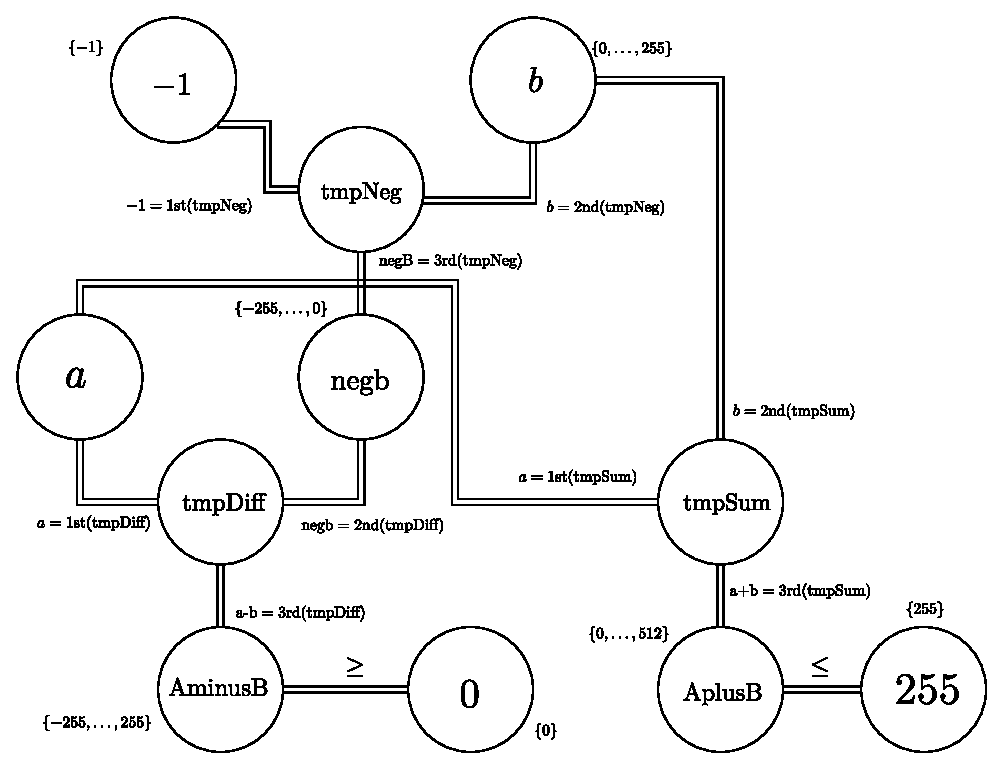
\includegraphics[width=0.7\linewidth]{pictures/Constraint_network.eps}
\caption{CSP graph example \cite{online:binarizationconstraint}.}
\label{fig:crv:graph}
\end{figure}

\subsubsection{Solving a CSP}
Generally, to solve a Constraint Satisfaction Problem, there are two types of
strategies \cite{tsang1999glimpse}. The first one, called \emph{systematic
search}, follows a linear process in which the algorithm tries to assign a value
to each variable while respecting each constraint until a solution is found. The
second group of strategies is a \emph{repair strategy}. This type of strategy
relies on assigning each variable a random value and checking if all the
constraints are respected. If one or more assignments do not respect the CSP
constraint, systematically, the algorithm tries to assign a different solution
to the variables that do not respect one or more constraints. This thesis
focuses on solving constraint satisfaction problems with a ``systematic search".

To solve a CSP with ``systematic search", the general incremental formulation as
a common search problem is the following \cite{russell2002artificial}:
\begin{description}
    \item[Initial state]: The initial state is an empty assignment in which all the variables are unassigned.
    \item[Next state function]: Search for a value that can be assigned to the next unassigned variable. The value should be consistent with the constraint declared in the problem.
    \item[Test Goal]:  Check if the assignment is complete. Otherwise, continue with the next step function.
\end{description}

An intrinsic property of every CSP is the max depth of the search. By
considering a CSP with $n$ number of variables, each complete assignment appears
at depth $n$ in the search tree, which implies that the systematic search
approach follows the structure of a depth-first search approach. If all the
domain $D_1 \dots, D_n$ have the same number of elements $d$, the branching
factor is equal to

\begin{equation}
b = (n - i) d
\end{equation}

Where $i$ is the current depth. This implies that the total amount of leaves is
\cite{Chowdhary2020}:

\begin{equation}
    \prod_{i=0}^{n-1}(n-i)d^n = n ! d^n
\end{equation}

As described above, the idea of ``systematic search" is to assign each variable
a value until it is compatible with the variable constraints and repeat this
process until a solution is found. In case no value is respecting the
constraint, the algorithm has to step back, remove the value assigned to the
last variable, and continue with a new value.

The process of stepping back is also known as backtracking. Backtracking alone
is the most basic form of ``systematic search". Contrary to state-space search
algorithms, which progress in only one direction, CSP algorithms have choices.
The choices are in the form of which successor variable to chose or a specific
type of inference called constraint propagation \cite{russell2002artificial} and
reducing the number of possible values that can be assigned to a variable, thus
reducing the choice considered in the next variable assignment. Constraint
propagation is a process that can be done while performing the search, or it can
be done before the search as a prepossessing step, which in some cases is
beneficial because it can solve the CSP and, therefore, no search is required.

One of the critical ideas is local consistency, like in figure
\ref{fig:crv:graph}, if we treat each variable as a node in a graph and each
constraint as an edge, then the process of enforcing local consistency in each
part of the graph causes inconsistent values to be eliminated from the domain of
the variables.

One of the most specific optimizations for solving a satisfaction problem is
node consistency. A single variable (corresponding to a node in the CSP graph)
is node-consistent if all the variable domain's values satisfy the variable's
unary constraints. It is easy to eliminate all the unary constraints in a CSP by
reducing the domain of variables with unary constraints at the start of the
solving process. An example of node consistency linked to listing
\ref{listing:unaryconstraintsv} would be the elimination of all the values above
100 for the domain of the variable \mints{a}.

When the CSP is node consistent it is possible to proceed with a second second
type of optimization, arc consistency.

\subsection{Arc Consistency}
A CSP variable is arc-consistent if every value in its domain satisfies the
variable's binary constraints. More formally, $v_i$ is arc-consistent concerning
another variable $v_j$ if for every value in the current domain $D_i$, there is
some value in the domain $D_j$ that satisfies the binary constraint on the edge
$(v_i, v_j)$.

Furthermore, a graph is arc-consistent if every variable is arc-consistent with
every other variable. Arc consistency can be obtained using different
algorithms, but the most popular and the one used in this thesis is AC-3. This
algorithm relies on a queue of arcs or constraints to consider line 1 algorithm
\ref{modifiedminibatch}. At the start of the procedure, the queue comprises all
the constraints specified in the direct and reverse traversing order. For
example, if there is a constraint between the variable \mints{a} and \mints{b}
such that \mints{a > b}. The queue will contain two elements, the first being
\mints{a > b} and the second \mints{b < a}.

The algorithm proceeds by removing from the queue one of the constraints $(v_i,
v_j)$ and makes each variable's domain consistent regarding $v_i$. If all the
values in the $D_i$ domain remain unchanged after this operation, the algorithm
continues to the next constraints. However, if this is not the case, it is
necessary to add to the queue all the arcs $(v_k, v_i)$ where $v_k$ are
neighbors of the current variable. The algorithm stops when the queue of
constraints is emptied. If a domain is revised to the empty domain, the
algorithm immediately terminates because there are no possible solutions.

The CSP obtained after revising the variables' domain by making it arc
consistent is equivalent to the starting CSP, but the search for a solution
would be much faster since fewer possible values are assignable to the set of
variables. There are specific cases in which the AC-3 procedure completely
solves the CSP by reducing the domain of each variable in the CSP to one
element.

The complexity of AC-3 can be analyzed by assuming a CSP composed of $n$
variables, each with a domain of size $d$ and $c$ binary constraints. Each
constraint or arc can be inserted at a maximum of $d$ times because that is the
maximum number of variables to delete for every single variable. Checking the
consistency of an arc can be done in $O(d^2)$ time, so the total worst-case time
is $O(cd^3)$ \cite{russell2002artificial}.

\begin{algorithm}
\caption{AC-3} \label{modifiedminibatch}
\begin{algorithmic}[1]
\Function{AC-3}{$\text{csp}$} \Return \textit{false} if an inconsistency is found and true otherwise
\State queue $\gets$ a queue of arcs, initially all the arcs in csp
\While {\textit{queue} is not empty} 
\State $(v_i, v_j) \gets \text{POP(queue)}$
\If {$\text{REVISE}(\text{csp}, v_i, v_j)$}
\If {$\text{size of}\; D_i = 0$}
\Return{\textit{false}}
\EndIf
\ForAll{$v_k \in v_i.\text{NEIGHBORS} - {v_j}$}
\State $\text{add} (v_k, v_i)$ to queue
\EndFor
\EndIf
\EndWhile
\State \Return{\textit{true}}
\EndFunction
\end{algorithmic}

\begin{algorithmic}[1]
\Function{REVISE}{$\text{csp}, v_i, v_j$} \Return \textit{true} if we revise the domain of $v_i$
\State $revised \gets \textit{false}$
\ForAll{$x \in D_i$}
\If{ $(x, y) \; \forall y \in D_j$ do not satisfy the constraint between $v_i, v_j$}
\State delete $x$ from $D_i$
\State $\textit{revised} \gets \textit{true}$
\EndIf
\EndFor
\State \Return{\textit{revised}}
\EndFunction
\end{algorithmic}
\end{algorithm}

At the end of the constraint propagation process, if the CSP is arc consistent,
but the assignment is not complete, and there are still variables with multiple
possible values, the algorithm has to continue searching for the next unassigned
variable. One of the most used algorithms for finding a partial assignment
solution is the backtracking algorithm explained in the next section.

\subsection{Backtracking}
Algorithm \ref{backtracking} shows the procedure known as backtracking. The
principle behind this procedure is that it repeatedly chooses an unassigned
variable then tries all values in that variable's domain in turn, trying to
extend each one into a solution via a recursive call. If the call succeeds, the
solution is returned, and if it fails, the assignment is restored to the
previous state, and the procedure tries the next value. In case the algorithm
tries all the values, and none of them works, it will return a failure.

\begin{algorithm}
\caption{BACKTRACKING-SEARCH} \label{backtracking}
\begin{algorithmic}[1]
\Function{BACKTRACKING-SEARCH}{$\text{csp}$} \Return a solution or \textit{failure}
\Return{BACKTRACK(csp, \{\})}
\EndFunction
\end{algorithmic}

\begin{algorithmic}[1]
\Function{BACKTRACK}{csp, assignment} \Return a solution or \textit{failure }
\If{\textit{assignment} is complete}
\State \Return \textit{assignemnt}
\EndIf
\ForAll{\textit{value} $\in$ ORDER-DOMAIN-VALUES(csp, var, assignment)}
    \If{\textit{value}, is consistent with \textit{assignment}}
        \State add $\{ \text{var} = \text{value}$ to \textit{assignment}\}
        \State \textit{inferences} $\gets$ INFERENCE(\textit{csp}, \textit{var}, \textit{assignment}
            \If{$\text{inferences} \neq \text{failure}$}
                \State add \textit{inference} to \textit{csp}
                \State \textit{result} $\gets$ BACKTRACK(\textit{csp}, \textit{assignment})
                \If{$\text{result} \neq \text{failure}$}
                    \State \Return \textit{result}
                \EndIf
                \State remove \textit{inferences} from \textit{csp}
            \EndIf
            \State remove $\{\text{var} = \text{value}\}$ from \textit{assignment}
    \EndIf
\EndFor
\State \Return \textit{failure}
\EndFunction
\end{algorithmic}
\end{algorithm}

\subsection{The language of constraints}
As stated in section \ref{sec:csp:def}, to fully describe a Constraint
Satisfaction Problem requires three fundamental quantities, a list of variables,
a domain for each of the variables, and a set of constraints applicable to the
variables.

Generally, the environment in which hardware design operates can be naturally
defined as a group of finite discrete domains. In this environment, variables
can have the form of Boolean, Signed, or Unsigned signals. For example, the ALU
defined in section \ref{sec:constrainedrandomsti} had three unsigned input with
a fixed with 8-bits for the (\mints{a}, \mints{b}) inputs and 2-bits for the
\mints{fn}. By defining the number of bits carried by each of the inputs, the
model implicitly defines the variables' domain. In this case, the maximum domain
for the two signed input (\mints{a}, \mints{b}) is all the integers number
between [0, 255] included. Finally, the third quantity, the constraint, can be
expressed with a new constructor that specifies the allowed values that each of
the random fields can take.

As shown in listing \ref{listing:3}, the result is a concise and expressive
class that can communicate all the required quantities in a compact form. The
ALU example is only a brief reference used to illustrate a possible way of
constraint programming. Going more in-depth by looking at the reference manual
of SystemVerilog \cite{ieee2017ieee}, it is clear that the syntax for describing
random objects is very exhaustive and can become quite complicated.

Challenged with creating a constraint programming environment for Chisel and
Scala, it was essential for the project to capture and reproduce the simplicity
of constraint programming present in SystemVerilog in the new library. The end
goal was not to simply create a library for solving constraints, there are
plenty of such libraries written in Java or other programming languages, but to
provide a tool to the user that integrates well with the Chisel development
environment.

One of the benefits of using a verification language with built-in constraint
satisfaction utilities like in SystemVerilog is the natural interoperability
between random objects and the whole environment. This natural interaction is
exceptionally significant because it allows writing very expressive test benches
and classes. The only way to achieve this interoperability between components is
to create a domain-specific language for constraints, which must be built on top
of Chisel and should coexist with it. From \cite{sutherland2003overview},
creating a parallel language was also the approach used by Accelera while
developing SystemVerilog.

Designing a new language allows us to model new technical properties more
straightforwardly and concisely describe the problem requirements. When creating
a new language, there are many aspects to consider. For this specific project,
the author focused on the consistency of the primitives provided by the language
while trying to maintain a syntax similar to SystemVerilog. In the next chapter,
F-CSP is introduced as the first attempt to create a library for solving
constraint satisfaction problems in Chisel.
